\section{A projektről TODO!}

A 3D nyomatás folyamat során rengeteg hiba bekövetkezhet,
melyek kihatnak a nyomtatott darab minőségére, anyagi kárt okoznak, súlyosabb esetben
a nyomató életébe is kerülhetnek. A folyamat valós idejű monitorizálásával, és 
jól tanított konvoluciós neurális hálózatok segítségével ezen hibák egy igen nagy része felismerhető.
A hibákat két kategóriába sorolnám: Nyomatás közben korrigálható, és azonnal félbeszakítandó hibák. 
A projekt célja egy olyan rendszer létrehozása, mely valós időben monitorizálja a 3D nyomatási folyamatot, minden lehetséges szögből,
Felismeri az adott hibát, és ennek megfelelően értesíti a felhasználót a teendőkről. Ezzel jelentős, költséget,
időt és nyersanyagot megspórolva a felhasználónak.

\subsection{Iparági relevancia és anyagspórlás}
A 3D nyomatás a jelenben már egy igen komoly iparággá nőtte, ki magát, tekintettel lévén arra, hogy 
Rengeteg új geometria megvalósítására nyitott kapukat, a gyártásban, és rendkívűl egyszerűvé tette a 
prototípus gyártást, ezzel gyorsítva a tömeggyártáshoz való eljutást. De miért is fontos a valós idejű monitorizálás?
Egy hobbiista, akinek egy nyomtató ül az asztalánál megengedheti magának, hogy időközönként ránézzen és közbelépjen
amenyiben ez indokolt, viszont az iparban, ahol egy nyomtatófarmon belül akár száz nyomtató is lehet ezt már
nem engedhetjük meg magunknak, automatizálni kell.

\begin{figure}[h]
    \centering
    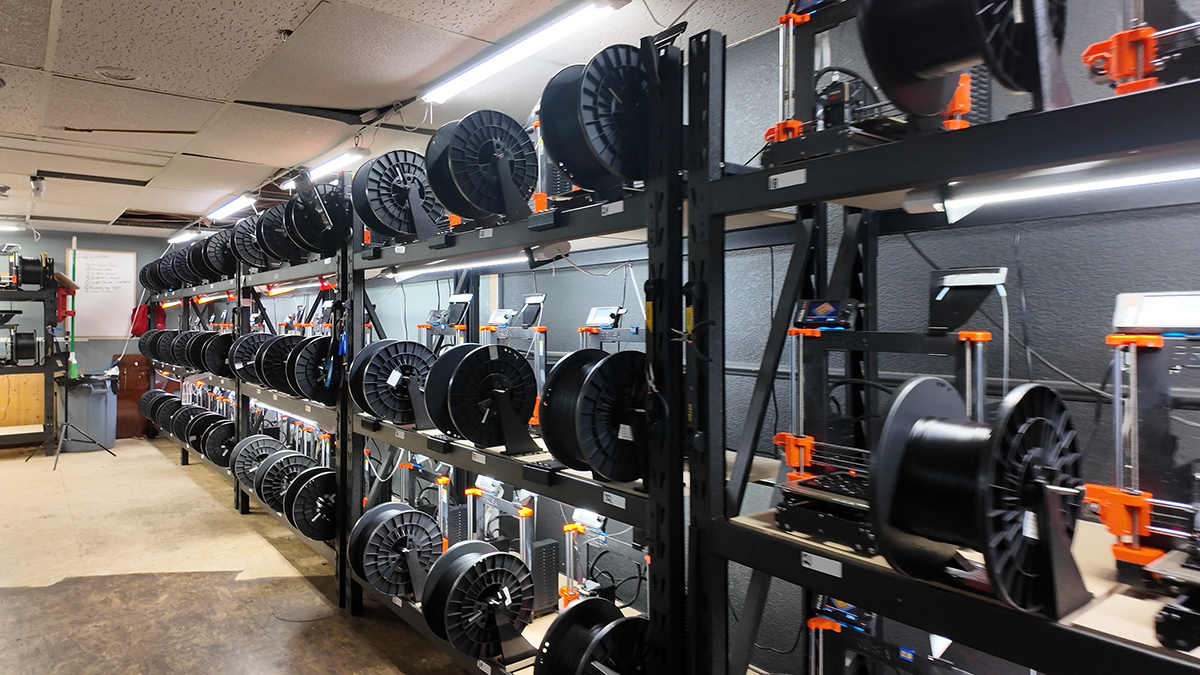
\includegraphics[width=\textwidth]{figures/images/literature/3dprintfarm.jpg}
    \caption{3D nyomtató farm}
\end{figure}

Egy ilyen farm esetén, már egy szeletelési hiba is, ha észrevétlen marad anyagi kárral, nyersanyagveszteséggel
vagy a berendezések sérülésével járhat.
A projekt keretein egy olyan skálázható rendszert szeretnénk megvalósítani, mely képes minden nyomtatón figyelni a darabokat, és
hiba kategóriának megfelelően jelezni amenyiben beavatkozásra van szükség. Az alapötlet: Egy olyan konvoluciós neuron háló
betanítása mely képes felismerni az alap hibákat, es ennek a beillesztése egy olyan keretrendszerbe, mely a nyomatott darabot több szemszögből figyeli.